% Compile using: TEXINPUTS=minted/source: pdflatex -shell-escape %
\documentclass[12pt,utf8,notheorems,compress,t]{beamer}
\usepackage{etex}

\usepackage[ngerman]{babel}

\usepackage{mathtools}
\usepackage{booktabs}
\usepackage{array}
\usepackage{ragged2e}
\usepackage{multicol}
\usepackage{xstring}
\usepackage{mathtools}
\usepackage{soul}\setul{0.2ex}{}
\usepackage{minted}
\usepackage[all]{xy}
\xyoption{rotate}
\usepackage{tikz}
\usetikzlibrary{calc,shapes.callouts,shapes.arrows}

\usepackage[protrusion=true,expansion=true]{microtype}

\hypersetup{colorlinks=true}

\newcommand{\NN}{\mathbb{N}}
\newcommand{\QQ}{\mathbb{Q}}
\renewcommand{\_}{\mathpunct{.}}
\newcommand{\?}{\,{:}\,}
\newcommand{\defeq}{\vcentcolon=}
\newcommand{\defeqv}{\vcentcolon\equiv}

\newcommand{\fmini}[2]{%
  \setlength{\fboxrule}{2pt}%
  \setlength{\fboxsep}{-3pt}%
  \usebeamercolor[fg]{item}\fbox{\usebeamercolor[fg]{normal text}\parbox{#1}{\begin{center}#2\end{center}}}}

\newcommand{\korr}[2]{
  \begin{center}
    \fmini{0.25\textwidth}{#1}
    {\usebeamercolor[fg]{item}$\boldsymbol{\xleftrightarrow{\qquad\quad}}$}
    \fmini{0.25\textwidth}{#2}
  \end{center}}
\newcommand{\pkorr}[2]{
  \begin{center}
    \parbox{0.25\textwidth}{\begin{center}#1\end{center}}
    %\parbox{0.5\textwidth}{\ \\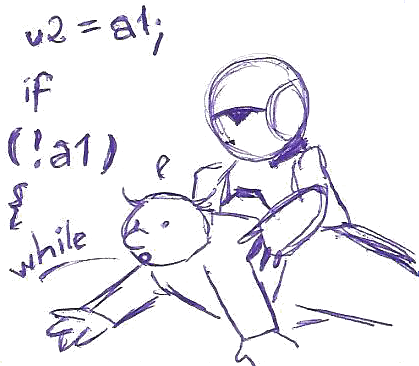
\includegraphics[scale=0.25]{images/program-extraction-without-border}}
    {\usebeamercolor[fg]{item}$\boldsymbol{\phantom{\xleftrightarrow{\qquad\quad}}}$}
    \parbox{0.25\textwidth}{\begin{center}#1\end{center}}
  \end{center}}

\setlength\parskip{\medskipamount}
\setlength\parindent{0pt}

\title{Konstruktive Mathematik, die Doppelnegationsübersetzung und Continuations}
\author{Ingo Blechschmidt}
\date{4. Dezember 2015}

\usetheme{Warsaw}
\usecolortheme{seahorse}
%\usefonttheme{default}?
%\usepackage{kurier}?
\usefonttheme{serif}
\usepackage[T1]{fontenc}
\usepackage{libertine}
%\usepackage{mathpazo}
\useinnertheme{rectangles}

\setbeamertemplate{blocks}[rounded][shadow=false]

\newenvironment{changemargin}[2]{%
  \begin{list}{}{%
    \setlength{\topsep}{0pt}%
    \setlength{\leftmargin}{#1}%
    \setlength{\rightmargin}{#2}%
    \setlength{\listparindent}{\parindent}%
    \setlength{\itemindent}{\parindent}%
    \setlength{\parsep}{\parskip}%
  }%
  \item[]}{\end{list}}

\newcommand{\slogan}[1]{%
  \begin{center}%
    \setlength{\fboxrule}{2pt}%
    \setlength{\fboxsep}{5pt}%
    {\usebeamercolor[fg]{item}\fbox{\usebeamercolor[fg]{normal text}\parbox{0.80\textwidth}{#1}}}%
  \end{center}%
}

\setbeamertemplate{frametitle}{%
  \vskip1em%
  \leavevmode%
  \begin{beamercolorbox}[dp=1ex,center]{}%
      \usebeamercolor[fg]{item}{\textbf{\Large \insertframetitle}}
  \end{beamercolorbox}%
}

\setbeamertemplate{headline}{}
\setbeamertemplate{navigation symbols}{}

\newcounter{framenumberpreappendix}
\newcommand{\backupstart}{
  \setcounter{framenumberpreappendix}{\value{framenumber}}
}
\newcommand{\backupend}{
  \addtocounter{framenumberpreappendix}{-\value{framenumber}}
  \addtocounter{framenumber}{\value{framenumberpreappendix}} 
}

\setbeamertemplate{footline}{%
  \begin{beamercolorbox}[wd=\paperwidth,ht=2.5ex,dp=1.25ex,right,rightskip=1mm,leftskip=1mm]{frametitle right}
    {\quad} \inserttitle \hfill \insertauthor \quad
    \insertframenumber\,/\,\inserttotalframenumber {\quad}
  \end{beamercolorbox}}

\newcommand{\hil}[1]{{\usebeamercolor[fg]{item}{\textbf{#1}}}}

\IfSubStr{\jobname}{\detokenize{notes}}{
  \setbeameroption{show notes}
}{
  \setbeameroption{hide notes}
}
\setbeamertemplate{note page}[plain]

\begin{document}

\begin{frame}[c]
  \centering
  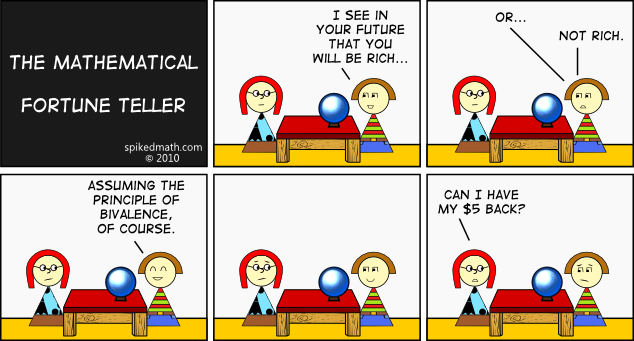
\includegraphics[scale=0.5]{images/fortune-teller}
  \medskip

  \hil{Konstruktive Mathematik, \\ die Doppelnegationsübersetzung und Continuations}
  \medskip

  \scriptsize
  Ingo Blechschmidt \\
  Universität Augsburg
  \medskip

  Haskell in Leipzig \\
  4. Dezember 2015
  \par
\end{frame}

\begin{frame}\frametitle{Gliederung}
  \small
  \tableofcontents
\end{frame}


\section{Konstruktive Mathematik}

\subsection{Ein Märchen über klassische Logik}

\begin{frame}[plain]\frametitle{Ein Märchen über klassische Logik}
  \vspace*{-1.5em}
  \begin{changemargin}{-1em}{-1em}
    \setlength{\columnsep}{15pt}
    \begin{multicols}{2}
      \justifying
      \scriptsize
      \textbf{Erzähler.}
Vor langer, langer Zeit begab sich im fernen, fernen Curry\-land folgende
Geschichte. Eines Tages holte die Königin des Landes und aller Haskellistas und
Lambdroiden ihren Haus- und Hof-Phi\-lo\-so\-phen zu sich.

\textbf{Königin.}
Philosoph! Ich habe folgenden Auftrag an dich: Beschaffe mir den Stein der
Weisen, oder alternativ finde heraus, wie man mithilfe des Steins unbegrenzt
Gold herstellen kann!

\textbf{Philosoph.}
Aber meine Königin! Ich habe nichts Brauchbares studiert! Wie soll ich diese
Aufgabe erfüllen?

\textbf{Königin.}
Das ist mir egal! Wir sehen uns morgen wieder. Erfüllst du deine Aufgabe nicht,
sollst du gehängt werden. Oder wir hacken deinen Kopf ab und verwenden ihn als
Cricket-Ball.

\textbf{Erzähler.}
Nach einer schlaflosen Nacht voller Sorgen wurde der Philosoph erneut zur
Königin berufen.

\textbf{Königin.}
Nun! Was hast du mir zu berichten?

\textbf{Philosoph.}
Ich habe es tatsächlich geschafft, herauszufinden, wie man den Stein verwenden
könnte, um unbegrenzt Gold herzustellen. Aber nur ich kann dieses Verfahren
durchführen, Eure Hoheit.

\textbf{Königin.}
Nun gut, dann sei es so!

\textbf{Erzähler.}
Und so vergingen die Jahre, in denen sich der Philosoph in Sicherheit wähnte
und die Angst vor Cricket-Schlägern langsam verlor. Die Königin suchte nun
selbst nach dem Stein, aber solange sie ihn nicht fand, hatte der Philosoph
nichts zu befürchten. Doch eines Tages passierte das Unfassbare: Die Königin hatte den Stein
gefunden! Und lies prompt den Philosophen zu sich rufen.

\textbf{Königin.}
Philosoph, sieh! Ich habe den Stein der Weisen gefunden, hier! Nun erfülle du
deinen Teil der Abmachung! \emph{[übergibt den Stein]}

\textbf{Philosoph.}
Danke. Ihr hattet von mir verlangt, Euch den Stein der Weisen zu beschaffen
oder herauszufinden, wie man mit ihm unbegrenzt Gold herstellen kann. Hier habt
Ihr den Stein der Weisen. \emph{[übergibt den Stein zurück]}

    \end{multicols}
  \end{changemargin}
\end{frame}

\note{\justifying\footnotesize
  Edward Yang erzählt in seinem
  \href{http://blog.ezyang.com/2013/04/a-classical-logic-fairy-tale/}{Blog}
  eine leichte Variante dieses Märchens. Es wurde von Philip Wadler in seinem
  \href{http://homepages.inf.ed.ac.uk/wadler/papers/dual/dual.pdf}{"`CbV is
  dual to CbN"'}-Aufsatz popularisiert und geht vielleicht auf Peter Selinger
  zurück.

  Wenn sich das Märchen "`continuation-y"' anfühlt, hat man schon eine gewisse
  Vorahnung, wohin die Reise geht.
  \par
}


\subsection{Das Axiom vom ausgeschlossenen Dritten}

\begin{frame}\frametitle{Nichtkonstruktive Beweise}
  Eine Zahl heißt genau dann \hil{rational}, wenn sie sich als Bruch zweier
  ganzer Zahlen schreiben lässt.
  \begin{itemize}
    \item $\frac{21}{13}$ und $37$ sind rational.
    \item $\sqrt{2}$ und $\pi$ sind irrational.
  \end{itemize}

  \only<1>{\vspace*{1em}\centering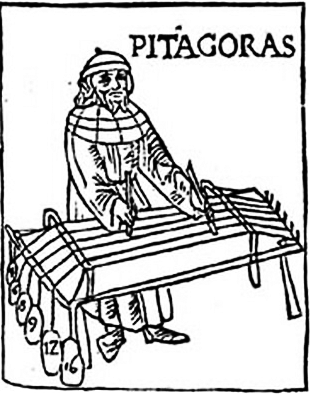
\includegraphics[scale=0.3]{images/pythagoras}}

  \pause

  \hil{Satz.} Es gibt \hil{irrationale} Zahlen~$x$ und~$y$ sodass~$x^y$ rational ist.
  \medskip

  \pause
  \hil{Beweis.} Entweder ist~$\sqrt{2}^{\sqrt{2}}$ rational oder nicht.
  \begin{enumerate}
    \item Im ersten Fall sind wir fertig.
    \item Im zweiten Fall können wir~$x \defeq \sqrt{2}^{\sqrt{2}}$ und~$y \defeq
  \sqrt{2}$ nehmen. Dann ist~$x^y = \sqrt{2}^{\sqrt{2} \cdot \sqrt{2}} =
  \sqrt{2}^2 = 2$ rational.
  \end{enumerate}
\end{frame}

\note{\justifying\footnotesize
  Der Beweis ist schön und kurz. Allerdings kennen wir nach dem Beweis immer noch
  nicht ein konkretes Beispiel für ein Paar irrationaler Zahlen, die potenziert
  eine rationale Zahl ergeben! Der Beweis war \emph{nichtkonstruktiv}.

  Wenn wir aus einem Beweis explizite Zeugen (witnesses) extrahieren möchten,
  muss der Beweis konstruktiv sein, zum Beispiel wie folgender:

  \begin{quote}Setze~$x \defeq \sqrt{2}$ und~$y \defeq \log_{\sqrt{2}} 3$.
  Dann ist~$x^y = 3$ rational. Der Beweis, dass~$y$ irrational ist, führt sich
  sogar leichter als der übliche Beweis, dass~$\sqrt{2}$ irrational
  ist.\end{quote}

  Es stellt sich heraus, dass von all den Axiomen klassischer Logik genau eines
  für Nichtkonstruktivität verantwortlich ist: das auf der nächsten Folie
  beschriebene Axiom vom ausgeschlossenen Dritten. In dem Beweis auf der
  vorherigen Folie ging es gleich in der ersten Zeile ein.
  \par
}

\newcommand{\constructiveinterpretation}{
  \begin{minipage}{0.99\textwidth}
    \begin{block}{\centering Konstruktive Interpretation}
      \begin{description}\small
        \item[$\bot$] Widerspruch.
        \item[$A \wedge B$] Wir haben Beleg für~$A$ und für~$B$.
        \item[$A \vee B$] Wir haben Beleg für~$A$ oder für~$B$.
        \item[$A \Rightarrow B$] Wir können Beleg für~$A$ in Beleg für~$B$
        transformieren.
        \item[$\forall x{:}X\_ A(x)$] Zu jedem $x:X$ können wir Beleg für
        $A(x)$ konstruieren.
        \item[$\exists x{:}X\_ A(x)$] Wir haben ein $x:X$ zusammen mit Beleg
        für~$A(x)$.
      \end{description}
    \end{block}
  \end{minipage}
}

\frame{\frametitle{Das Axiom vom ausgeschlossenen Dritten}
  \centering
  "`Für jede Aussage~$A$ dürfen wir~$A \,\vee\, \neg A$ voraussetzen."'

  \medskip
  Klassische Logik $=$ \\
  konstruktive Logik $+$ das Axiom vom ausgeschlossenen Dritten.

  \vfill

  \only<1>{
    \centering
    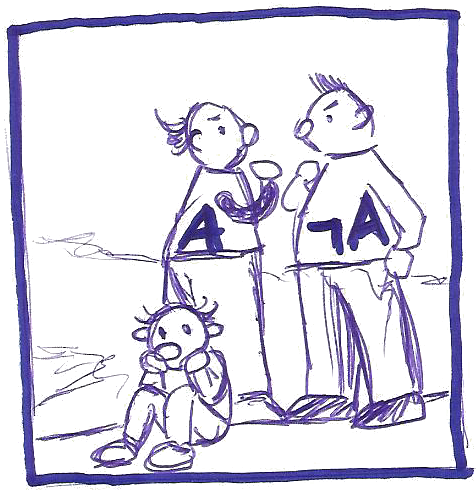
\includegraphics[scale=0.7]{images/lem}
    \par
  }

  \only<2>{
    \centering
    \begin{minipage}{0.8\textwidth}
      \begin{block}{\centering Klassische Interpretation}
        \begin{description}\small
          \item[$\bot$] Widerspruch.
          \item[$A \wedge B$] $A$ und $B$ sind wahr.
          \item[$A \vee B$] $A$ ist wahr oder $B$ ist wahr.
          \item[$A \Rightarrow B$] Sollte $A$ wahr sein, so auch $B$.
          \item[$\forall x{:}X\_ A(x)$] Für alle $x:X$ gilt $A(x)$.
          \item[$\exists x{:}X\_ A(x)$] Es gibt ein $x:X$ mit $A(x)$.
        \end{description}
      \end{block}
    \end{minipage}
    \par
  }
}


\subsection{Die konstruktive Interpretation logischer Symbole}

\begin{frame}\frametitle{Klassische vs. konstruktive Logik}
  \vspace*{-0.5em}
  \small
  \setlength{\extrarowheight}{0.6em}
  \begin{tabular}{@{$\!\!\!\!\!\!$}lll}
    \hil{Symbol} & \hil{klassisch} & \hil{konstruktiv} \\
    $\bot$ & Widerspruch. & Widerspruch. \\
    $A \wedge B$ & $A$ und $B$ sind wahr. & Wir haben Beleg für~$A$ und für~$B$. \\
    $A \vee B$ & $A$ ist wahr oder $B$ ist wahr. & Wir haben Beleg für~$A$ oder für~$B$. \\
    $A \Rightarrow B$ & Aus~$A$ folgt~$B$. & Wir können Beleg für~$A$ in \\[-0.8em]&& Beleg für~$B$ transformieren. \\
    $\forall x{:}X\_ A(x)$ &
    Für alle $x:X$ gilt $A(x)$. &
    Zu jedem $x:X$ können wir \\[-0.8em]&&
    Beleg für $A(x)$ konstruieren. \\
    $\exists x{:}X\_ A(x)$ &
    Es gibt ein $x:X$ mit $A(x)$. &
    Wir haben ein $x:X$ zusammen \\[-0.8em]&&
    mit Beleg für~$A(x)$. \\
    \pause
    $\neg A$ & $A$ ist falsch. & Es gibt keinen Beleg für $A$. \\
    $\neg\neg A$ & $A$ ist nicht nicht wahr. & Es gibt keinen Beleg für $\neg A$.
  \end{tabular}
\end{frame}

\note{\justifying\footnotesize
  In der konstruktiven Mathematik verwendet man dieselben logischen Symbole wie in der
  klassischen Mathematik, versieht sie aber mit einer leicht anderen Bedeutung.
  Die klassische Interpretation des Axioms vom ausgeschlossenen Dritten ist
  einfach die, dass jede Aussage wahr oder falsch ist. Da es hier nur um
  mathematische (also in einem starken Sinn objektive) Aussagen geht, ist das
  eine banale Trivialität: Entweder gibt es unendlich viele Primzahlzwillinge
  oder eben nicht. [Es gibt auch die Philosophie, das Axiom vom
  ausgeschlossenen Dritten auch auf Meta-Ebene abzulehnen. Darum geht es hier
  aber nicht.]

  Die konstruktive Interpretation dagegen lautet: Für jede Aussage~$A$ haben
  wir entweder Beleg für~$A$ oder für~$\neg A$. Das ist eine absurde
  Behauptung. (Man erinnere sich an Gödels Unvollständigkeitssatz: Es gibt
  Aussagen -- \emph{Gödelsätze} -- die die Eigenschaft haben, dass weder sie
  noch ihre Negation beweisbar sind.)

  Mit "`wir"' in der Tabelle ist nicht wortwörtlich irgendeine Gruppe von
  Leuten gemeint; es sollte in einem generischen mathematischen Sinn gelesen
  werden. Stichwörter sind die \emph{Brouwer--Heyting--Kolmogorov-Interpretation}
  und \emph{Realisierbarkeitstheorie} (siehe zum Beispiel
  \href{http://math.andrej.com/data/c2c.pdf}{Notizen von Andrej Bauer}).

  Die Notation~"`$\neg A$"' für die Negation ist \emph{syntaktischer Zucker}
  für~"`$A \Rightarrow \bot$"'.
  
  Aus einer Aussage~$A$ folgt konstruktiv wie klassisch ihre doppelte
  Negation~$\neg\neg A$, aber konstruktiv gilt im Allgemeinen nicht die
  Umkehrung.
  \par
}

\note{\justifying\footnotesize
  Vor ein paar Jahren tauchte ein Video von Kate Moss auf, das sie beim
  Konsumieren von Drogen zeigte. Aus dem Video war klar, dass es sich dabei entweder um
  Drogen von einem gewissen Typ~$A$ oder von einem gewissen Typ~$B$ handelte;
  aber es gab keinen direkten Beleg für einen der beiden Typen.
  Kate Moss wurde nicht verfolgt; in diesem Sinn verwendete das Justizsystem
  also konstruktive Logik. Siehe
  \href{http://blog.sigfpe.com/2008/06/drugs-kate-moss-and-intuitionistic.html}{ein
  Blog-Post von Dan Piponi} über das Thema.

  Konstruktive Logik kann feinere Unterschiede abbilden als klassische Logik.
  Wenn wir zum Beispiel wissen, dass sich unser Haustürschlüssel irgendwo in
  der Wohnung befinden muss (da wir ihn letzte Nacht verwendet haben, um die Tür
  aufzusperren), wir ihn momentan aber nicht finden, so können wir konstruktiv
  nicht die Aussage vertreten, dass es eine Stelle gäbe, an der der Schlüssel
  liege. Denn dazu müssten wir in der Lage sein, einen expliziten Zeugen dieser
  Existenzbehauptung (also den Aufenthaltsort des Schlüssels) anzugeben.
  Wir können konstruktiv nur die durch doppelte Negation abgeschwächte Aussage
  vertreten.

  (Die Beispiele hinken etwas, da sie sich auf den Kenntnisstand von gewissen
  Personen beziehen.)
  \par
}

\note{\justifying\footnotesize
  Nebenbei bemerkt: Konstruktive MathematikerInnen behaupten \emph{nicht}, dass
  das Axiom vom ausgeschlossenen Dritten falsch sei (d.\,h. dass seine Negation
  gelten würde). Sie setzen es nur nicht in seiner vollen Allgemeinheit voraus.

  Tatsächlich lassen sich manche Instanzen des Axioms auch konstruktiv zeigen:
  Zum Beispiel folgt mit Induktion, dass jede natürliche Zahl gleich Null oder
  ungleich Null ist. (Die analoge Behauptung für reelle Zahlen lässt sich
  konstruktiv nicht zeigen. Das hat eine Parallele in der Programmierung:
  Bekanntlich ist es unschicklich, Fließkommazahlen auf Gleichheit zu testen,
  während das bei Ganzzahlen kein Problem ist.)

  An dieser Stelle sollte auch das mancherorts immer noch geisternde Gerücht
  zerstreut werden, dass in konstruktiver Mathematik das Wort
  \emph{Widerspruch} grundsätzlich verboten wäre. Das stimmt so nicht; wenn man
  die Situation genauer verstehen möchte, muss man den Unterschied zwischen
  \emph{Beweisen von negierten Aussagem} und echten \emph{Widerspruchsbeweisen}
  verstehen. Das erklärt
  Andrej Bauer
  \href{http://math.andrej.com/2010/03/29/proof-of-negation-and-proof-by-contradiction/}{auf
  seinem Blog} ganz wunderbar.
  \par
}

\note{\justifying\footnotesize
  Zwei letzte Bemerkungen. PhilosophInnen untersuchen nicht nur was \emph{wahr} ist,
  sondern auch was stimmen \emph{sollte}, was \emph{möglich} ist, was \emph{notwendig} ist, was
  jemand \emph{weiß} oder was jemand \emph{glaubt}. Das formalisiert man mit \emph{modalen
  Operatoren}.

  Als MathematikerIn kann man daher manchmal neidisch werden. In konstruktiver
  Mathematik aber gibt es durchaus eine Vielzahl von modalen Operatoren! Die
  Doppelnegation ist das wichtigste Beispiel. (In klassischer Logik ist die
  Doppelnegation auch ein modaler Operator, dort aber ein sehr
  uninteressanter.)

  Es gibt mehrere gute und von philosophischen Vorlieben unabhängige Gründe,
  konstruktive Mathematik zu untersuchen. Einer steht auf der übernächsten Folie:
  die Curry--Howard-Korrespondenz funktioniert nur mit konstruktiven Beweisen.
  Ein anderer ist, dass nur konstruktive Logik allen \emph{Topoi} --
  mathematischen Alternativuniversen -- gemein ist.

  Wer sich von einer mathematischen Sicht näher für das Thema interessiert, kann in ein
  \href{http://pizzaseminar.speicherleck.de/skript2/konstruktive-mathematik.pdf}{Skript
  zu einem Pizzaseminar} schauen.
  \par
}


\subsection{Die Doppelnegationsübersetzung}

\newcommand{\inegneg}{{\usebeamercolor[fg]{item}{\boldsymbol{\neg\neg}}}}
\newcommand{\gnegneg}[1]{\textcolor{gray}{\boldsymbol{\neg\neg}(}#1\textcolor{gray}{)}}

\begin{frame}\frametitle{Die Doppelnegationsübersetzung}
  \vspace*{-2em}
  \begin{align*}
    (x=y)^\Box &\defeqv \inegneg (x=y) \\
    (A \wedge B)^\Box &\defeqv \gnegneg{A^\Box \wedge B^\Box} \\
    (A \vee B)^\Box &\defeqv \inegneg(A^\Box \vee B^\Box) \\
    (A \Rightarrow B)^\Box &\defeqv \gnegneg{A^\Box \Rightarrow B^\Box} \\
    (\forall x{:}X\_ A(x))^\Box &\defeqv \gnegneg{\forall x{:}X\_ A^\Box(x)} \\
    (\exists x{:}X\_ A(x))^\Box &\defeqv \inegneg(\exists x{:}X\_ A^\Box(x))
  \end{align*}

  Beispiel: Die Doppelnegationsübersetzung von
  \begin{center}
    \emph{Es gibt eine Stelle, an der der Schlüssel liegt.}
  \end{center}
  \vspace*{-0.8em}
  ist
  \vspace*{-0.5em}
  \begin{center}
    \emph{Es gibt \hil{nicht nicht} eine Stelle, an der der Schlüssel
    liegt.}
  \end{center}

  \hil{Satz.} Es gilt $A$ genau dann klassisch, wenn $A^\Box$ konstruktiv gilt.
\end{frame}

\note{\justifying\footnotesize
  Die grauen~\textcolor{gray}{$\neg\neg$}'s können weggelassen werden. Die
  blauen~$\inegneg$'s dagegen sind entscheidend; man könnte sagen, dass der
  einzige Unterschied zwischen klassischer und konstruktiver Logik in der
  Bedeutung der Disjunktion und des Existenzquantors liegen.

  Siehe ein
  \href{http://pizzaseminar.speicherleck.de/skript2/konstruktive-mathematik.pdf}{Skript
  zu einem Pizzaseminar} für Details zur Doppelnegationsübersetzung.

  Die grundlegende Beweisidee werden wir im Laufe der Folien noch verstehen.
  \par
}


\section{Die Curry--Howard-Korrespondenz}

\subsection{Eine Brücke zwischen Logik und Programmierung}

\begin{frame}\frametitle{Die Curry--Howard-Korrespondenz}
  \korr{\hil{Aussagen}}{\hil{Typen}}
  \vspace*{-3em}
  \pkorr{\usebeamercolor[fg]{item}$\boldsymbol{\Biggl|}$}{\usebeamercolor[fg]{item}$\boldsymbol{\Biggl|}$}
  \vspace*{-3em}
  \korr{\hil{Beweise}}{\hil{Terme}}

  \only<1>{
    \centering
    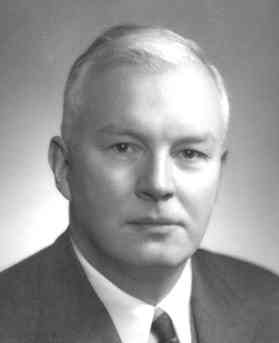
\includegraphics[height=2.2cm]{images/haskell-curry}
    \qquad
    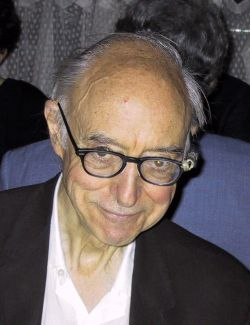
\includegraphics[height=2.2cm]{images/william-howard}
    \par
  }

  \only<2>{
    \centering
    \setlength{\extrarowheight}{0.3em}
    \begin{tabular}{l@{\qquad}l}
      \hil{Logik} & \hil{Programmierung} \\
      $A \Rightarrow A$ & \texttt{A $\to$ A} \\
      $(A \wedge B) \Rightarrow A$ & \texttt{(A,B) $\to$ A} \\
      $A \Rightarrow (A \vee B)$ & \texttt{A $\to$ Either A B}
    \end{tabular}
    \par
  }
\end{frame}

\begin{frame}\frametitle{Die Curry--Howard-Korrespondenz}
  \centering
  \small
  \vspace*{-0.5em}
  \setlength{\extrarowheight}{0.3em}
  \begin{tabular}{l@{\qquad}l}
    \hil{Logik} & \hil{Programmierung} \\
    Aussage $A$ & Typ \texttt{A} der Belege für $A$ \\
    Beweis von $A$ & Programm vom Typ \texttt{A} \\
    $A \Rightarrow A$ & \texttt{A $\to$ A} \\
    $(A \wedge B) \Rightarrow A$ & \texttt{(A,B) $\to$ A} \\
    $A \Rightarrow (A \vee B)$ & \texttt{A $\to$ Either A B} \\
    $A \Rightarrow B$ & \texttt{A $\to$ B} \\
    \text{Es gibt eine natürliche Zahl.} & \texttt{Nat} \\
    \visible<2->{$\neg A$\visible<3->{, d.\,h. $A \Rightarrow \bot$} &
      \only<2-3>{??}%
      \visible<4->{\texttt{A $\to$ r}}} \\
    \visible<5->{$\neg\neg A$, d.\,h. $(A \Rightarrow \bot) \Rightarrow \bot$} &
      \only<5>{??}%
      \visible<6->{\texttt{(A $\to$ r) $\to$ r}}
  \end{tabular}
  \par

  \slogan{
    Aus jedem konstruktiven Beweis kann man ein Programm extrahieren.
    Jedes Programm beweist eine Behauptung.
  }
\end{frame}

\note{\justifying\footnotesize
  Die Curry--Howard-Korrespondenz schlägt eine erstaunliche und tief reichende
  Brücke zwischen konstruktiver Mathematik und Programmierung. Zu jeder
  logischen Aussage gehört ein Typ, anschaulich vorgestellt als der Typ ihrer
  Belege. Zu jedem konstruktiven Beweis der Aussage gehört ein Wert des
  entsprechenden Typs.

  Zu einer falschen Aussage gehört dann einfach der leere Typ, der keinerlei
  Werte hat. Etwa ist die Aussage "`aus~$A$ folgt~$B$"' im Allgemeinen falsch,
  und passend dazu ist der Typ~\texttt{A $\to$ B} im Allgemeinen unbewohnt
  (wenn man von \texttt{unsafeCoerce} und Nichtterminierung absieht).

  Das andere Extrem ist die Aussage "`Es gibt eine natürliche
  Zahl."', für die jede natürliche Zahl jeweils ein Beleg ist. Der Typ der
  Belege dieser Aussage ist also der Typ der natürlichen Zahlen.

  Die Curry--Howard-Korrespondenz ist fundamental auf konstruktive Beweise
  beschränkt.

  Für eine formale Behandlung muss man sowohl die linke Seite ("`Logik"') als
  auch die rechte ("`Programmierung"') konkretisieren. Eine Möglichkeit ist
  \emph{propositionale intuitionistische Logik} als linke und das
  \emph{einfach-getypte Lambda-Kalkül} als rechte Seite.
  \par
}

\note{\justifying\footnotesize
  Unter der Curry--Howard-Korrespondenz gehört zur Negation~$\neg A$ der
  Typ \texttt{A $\to$ r}. Das stellt man sich vor: Wenn man konstruktiv~$\neg
  A$ behauptet, so behauptet man, aus einem hypothetischen Beleg für~$A$ Beleg
  einer beliebigen anderen Aussage machen zu können. Schließlich glaubt man ja,
  dass es gar keinen Beleg für~$A$ gibt, sodass man also überzeugt ist, nie in
  die Verlegenheit zu geraten, diese Transformation durchführen zu müssen.

  Mit der Curry--Howard-Korrespondenz ist auch klarer, was der semantische
  Gehalt einer doppelt negierten Aussage ist. Unter der Korrespondenz gehört
  zur Aussage~$\neg\neg A$ der Typ~\texttt{(A $\to$ r) $\to$ r}, also einfach~\texttt{Cont r A}. Ein Wert dieses Typs kann
  zum Beispiel von der Form~\texttt{return x} sein, wobei~\texttt{x} ein Wert
  vom Typ~\texttt{A} ist. Ein Wert dieses Typs kann aber auch eine andere Form
  haben -- er kann mit der gegebenen Continuation spielen, zum Beispiel sie
  mehrmals ausführen.

  Etwas unpräzise ausgedrückt kann man sich merken: Eine doppelt negierte
  Aussage~$\neg\neg A$ konstruktiv zu belegen bedeutet, die Aussage~$A$
  \emph{innerhalb der Continuation-Monade}, also etwa unter Verwendung von
  Zeitsprüngen in die Vergangenheit, zu belegen.
  \par
}


\subsection{Doppelnegationsübersetzung $=$ CPS-Transformation}

\begin{frame}[fragile]\frametitle{$\boldsymbol{\neg\neg}$-Übersetzung $\widehat=$ CPS-Transformation}
  \begin{changemargin}{-0.3em}{0em}
    \centering
    \vspace*{-1em}
    \setlength{\extrarowheight}{0.3em}
    \begin{tabular}{@{}l@{\qquad}l}
      \hil{Logik} & \hil{Programmierung} \\
      Aussage $A$ & Typ \texttt{A} der Belege für $A$ \\
      Beweis von $A$ & Programm vom Typ \texttt{A} \\
      $\neg\neg A$, d.\,h. $(A \Rightarrow \bot) \Rightarrow \bot$ &
        \texttt{(A $\to$ r) $\to$ r}, d.\,h. \texttt{Cont r A} \\
      Doppelnegationsübersetzung & CPS-Transformation
    \end{tabular}

    \begin{minted}{haskell}
type Cont r a = ((a -> r) -> r)

-- Axiom vom ausgeschlossenen Dritten ohne Übersetzung:
-- lem :: Either a (a -> r)

lem :: Cont r (Either a (a -> Cont r b))
lem = \k -> k $ Right $ \x -> (\k' -> k (Left x))
    \end{minted}
  \end{changemargin}
\end{frame}

\note{\justifying\footnotesize
  Mit den Übersetzungsregeln der Curry--Howard-Korrespondenz entspricht zur
  Aussage~$A \vee \neg A$ der Typ~\texttt{Either A (A $\to$ r)}. Dieser ist im
  Allgemeinen nicht bewohnt, passend dazu, dass sich konstruktiv das Axiom vom
  ausgeschlossenen Dritten nicht zeigen lässt.
  
  Die Doppelnegationsübersetzung des Axioms vom ausgeschlossenen Dritten lässt
  sich aber sehr wohl konstruktiv zeigen. Das zeigt der auf der vorherigen
  Folie angegebene Term~\texttt{lem}.

  Es gibt übrigens mehrere Möglichkeiten, aus einem klassischen Beweis einer
  Aussage einen konstruktiven Beweis der übersetzten Aussage zu machen. Diese
  Möglichkeiten entsprechen den unterschiedlichen Varianten der
  CPS-Transformation (call by name, call by value, \ldots).
  \par
}

\note{\justifying\footnotesize
  Wie funktioniert das Programm~\texttt{lem}? Zunächst sichern wir uns die
  aktuelle Continuation~\texttt{k}. Dann behaupten wir sofort: "`Die Aussage
  ist falsch!"' Beziehungsweise: "`Es gibt keine Werte vom Typ~\texttt{a}!"'
  Wir geben also~\texttt{Right f} zurück, mit~\texttt{f} vom Typ~\texttt{a $\to$
  Cont r b}.  Diese Funktion~\texttt{f} ist der Zeuge für unsere Behauptung.

  Nun kann es zufälligerweise sein, dass unsere Behauptung richtig ist. Dann
  wird~\texttt{f} nie aufgerufen. Es kann aber auch sein, dass der Aufrufer
  einen Wert~\texttt{x} vom Typ~\texttt{a} auftreibt und damit unseren Bluff
  herausfordert. Natürlich ist es uns nicht möglich, mit einem Wert vom
  Typ~\texttt{b} aufzuwarten (über diesen wissen wir ja nichts weiter). Wir befreien
  uns aus unserer Not, indem wir die momentan laufende Berechnung abbrechen und
  die anfangs gesicherte Continuation nehmen. Dieser übergeben wir gerade den
  uns präsentierten Wert~\texttt{x}.

  Das ist auch genau die Strategie, die der Philosoph aus dem Märchen vom
  Anfang verfolgen sollte. Bei wörtlicher Auslegung der Geschichte nimmt er ja
  die Königin etwas auf den Arm, was sie vermutlich nicht gutheißen wird.
  Er sollte stattdessen, sobald er von der Königin den Stein der Weisen
  ausgehändigt bekommen hat, zurück in die Vergangenheit springen, zu jenem
  verhängnisvollen Tag, an dem die Königin den Philosophen das erste Mal zu
  sich rief.
  \par
}


\subsection{Fallbeispiel: Minima unendlicher Listen}

\begin{frame}[fragile]\frametitle{Minima unendlicher Listen}
  \hil{Satz.} In jeder unendlichen Liste~\texttt{xs} natürlicher Zahlen gibt es
  ein kleinstes Element.

  Aber nicht konstruktiv! Es gibt kein Programm vom Typ:
  \begin{center}
    \begin{minipage}{0.65\textwidth}
      \begin{minted}{haskell}
minimum :: [Nat] -> Ix
-- Ix: Typ der Indizes (also Nat)
      \end{minted}
    \end{minipage}
  \end{center}

  \pause
  \hil{Beweis.} Durch noethersche Induktion über die Größe eines gegebenen
  Elements~\texttt{xs!!i}.
  Entweder gibt es einen Index~\texttt{j} mit \texttt{xs!!j < xs!!i} oder nicht.
  \begin{enumerate}
    \item Im ersten Fall gibt es ein Minimum nach Ind'voraussetzung.
    \item Im zweiten Fall ist \texttt{xs!!i} minimal.
  \end{enumerate}
\end{frame}

\begin{frame}[fragile]\frametitle{Minima unendlicher Listen}
  \only<2>{\footnotesize\vspace*{-1.5em}}
  \begin{minted}{haskell}
type Cont r a = ((a -> r) -> r)

lem :: Cont r (Either a (a -> Cont r b))
lem = \k -> k $ Right $ \x -> (\k' -> k (Left x))

minimum :: [Nat] -> Cont r (Ix, Ix -> Cont r ())
minimum xs = go 0 where
   go i = do
      oracle <- lem
      case oracle of
         Left  j -> go j
         Right f -> return (i, \j ->
            if xs!!j >= xs!!i then return () else f j)
  \end{minted}
  \pause
  \begin{minted}{haskell}
example = do
   (i, g) <- minimum [...]
   g 5 >> g 7 >> g 3
   ...
  \end{minted}
\end{frame}

\note{\justifying\footnotesize
  Die angegebene Funktion~\texttt{minimum} berechnet (innerhalb der
  Continuation-Monade) das Minimum einer unendlichen Liste von natürlichen
  Zahlen. Ihr Rückgabewert ist ein Tupel~\texttt{(i, g)} bestehend aus dem
  Index~\texttt{i} des minimalen Elements und einem Zeugen~\texttt{g} seiner
  Minimalität: Gegeben ein weiterer Index~\texttt{j}, so soll~\texttt{g j}
  einen Beweis der Behauptung~\texttt{xs!!j >= xs!!i} zurückgeben.

  Um das treu umsetzen zu können, bräuchten wir abhängige Typen. Da es die in
  Haskell nicht gibt, muss der Unit-Typ~\texttt{()} zusammen mit einem sozialen
  Versprechen als Ersatz herhalten.
  \par
}

\note{\justifying\footnotesize
  Wie geht die Funktion~\texttt{minimum} in der Praxis vor? Um eigene Fehler
  später korrigieren zu können, sichert sie zunächst die aktuelle Continuation.
  Anschließend proklamiert sie das erste Listenelement (Index~\texttt{0}) als
  Minimum. Das kann tatsächlich korrekt sein. Falls allerdings
  irgendwann~\texttt{g} mit einem Index~\texttt{j}, für den~\texttt{xs!!j <
  xs!!i} ist, aufgerufen wird, so nimmt sie die eingangs gesicherte
  Continuation und sorgt so dafür, dass es den Anschein hat, als hätte sie die
  gesamte Zeit über behauptet, das Element~\texttt{xs!!j} sei das Minimum. Auf
  dieselbe Art und Weise geht es weiter.

  Von innerhalb der Continuation-Monade aus kann dieses Schummeln nicht
  beobachtet werden.
  
  Man muss allerdings beim Verlassen der Monade Sorgfalt
  walten lassen: Je nach konkretem Einsatzszenario kann es schlimm sein oder auch
  nicht, dass die Funktion nicht das tatsächlich minimale Element bestimmt, sondern nur
  das kleinste unter allen vom Rest des Programms inspizierten Elementen.
  \par
}

\note{\justifying\footnotesize
  Spannend ist noch, dass die Funktion~\texttt{minimum} \emph{nicht} das
  Ergebnis einer kreativen Überlegung ist. Stattdessen ergibt sich die Funktion
  rein mechanisch, indem man zunächst den nur in klassischer Logik gültigen
  Beweis des besprochenen Satzes mit der Doppelnegationsübersetzung in einen
  konstruktiven Beweis überführt und anschließend diesen mit der
  Curry--Howard-Korrespondenz zu einem Programm transformiert.

  Die Struktur des klassischen Beweises kann man in dem Programmcode deutlich
  erkennen. Der Aufruf von~\texttt{lem} steht sowohl im Code als auch im Beweis
  ganz am Anfang. Der \texttt{Left}-Fall im Code entspricht Fall~1 im Beweis.
  Der Beweis verwendete in diesem Fall die Induktionsvoraussetzung; das äußert
  sich im Code durch den rekursiven Aufruf~\texttt{go j}.

  Der \texttt{Right}-Fall im Code entspricht Fall~2 im Beweis. Dieser war auf
  der Folie verkürzt wiedergegeben; ausführlich lautet er so (ja, das ist etwas
  umständlich formuliert): "`Um zu beweisen, dass~\texttt{xs!!i} minimal ist,
  sei ein beliebiger Index~\texttt{j} gegeben. Wir müssen zeigen,
  dass~\texttt{xs!!j $\geq$ xs!!i}. Falls dem so sein sollte (diese
  Fallunterscheidung können wir konstruktiv treffen), sind wir fertig.
  Andernfalls gilt also~\texttt{xs!!j < xs!!i}. Das ist ein Widerspruch zur
  Fallvoraussetzung. Nach dem Explosionsprinzip folgt aus diesem Widerspruch
  unsere Behauptung."' Die Ähnlichkeit zum Code ist offenkundig; der Anwendung
  des Explosionsprinzips nach dem Herleiten des Widerspruchs entspricht dem
  Aufruf~\texttt{f j}.
  \par
}

\note{\justifying\tiny
  \setlength{\columnsep}{25pt}
  \begin{multicols}{2}
    Hier folgt noch ein praktisches Beispiel aus algorithmischer Zahlentheorie
    für die Nützlichkeit dieses "`algorithmischen Axioms vom ausgeschlossenen
    Dritten"'. Es soll demonstrieren, dass das schummelnde Verhalten in manchen
    Fällen völlig ausreicht.

    Sei~$x$ eine algebraische Zahl, also eine komplexe Zahl, die Nullstelle eines
    normierten Polynoms~$f(X) \in \QQ[X]$ ist. Dann gibt es die von~$x$ erzeugte
    Körpererweiterung~$\QQ(x)$ von~$\QQ$; dieser Körper enthält die rationalen
    Zahlen, die Zahl~$x$ und alle Zahlen, die induktiv aus diesen durch Addition,
    Subtraktion, Multiplikation und Division gewonnen werden können.

    Wir möchten einen Algorithmus dafür angeben, ein von Null verschiedenes
    Element in~$\QQ(x)$ zu invertieren und das Inverse als polynomiellen Ausdruck
    in~$x$ anzugeben. Theoretisch funktioniert das wie folgt:

    Zunächst zerlegen wir~$f(X)$ in seine irreduzible Faktoren. Einer der
    Faktoren, sagen wir~$g(X)$, hat immer noch~$x$ als Nullstelle. Dieser Faktor
    heißt auch \emph{Minimalpolynom} von~$x$, und die allgemeine Theorie besagt,
    dass~$\QQ(x)$ isomorph zum Ring~$\QQ[X]/(g(X))$ ist. Das heißt:
    In~$\QQ(x)$ zu arbeiten ist gleichbedeutend damit, im Polynomring~$\QQ[X]$
    modulo~$g(X)$ zu arbeiten. Von diesem weiß man, dass der erweiterte
    euklidische Algorithmus ein effizientes Verfahren zur Bestimmung von
    modularen Inversen ist.

    Allerdings hat dieses Verfahren ein gravierendes Problem: Die Zerlegung
    von~$f(X)$ in seine irreduziblen Faktoren ist sehr aufwendig. Kann man die
    Zerlegung irgendwie umgehen?

    Ja! Sei~$[h(X)] \in \QQ[X]/(f(X))$. Wir möchten das Inverse von~$h(x)$
    in~$\QQ(x)$ bestimmen. Da~$f(X)$ nicht notwendigerweise irreduzibel ist, ist
    der Ring~$\QQ[X]/(f(X))$ nicht notwendigerweise ein Körper (jeder Faktor
    von~$f(X)$ ist in ihm ein Nullteiler). Wir können aber trotzdem den
    erweiterten euklidischen Algorithmus verwenden, um den (monischen) größten
    gemeinsamen Teiler~$d(X)$ von~$f(X)$ und~$h(X)$ und eine
    \emph{Bézoutdarstellung}
    \[ d(X) = a(X) f(X) + b(X) h(X). \]
    zu berechnen. Dann können drei Fälle eintreten:
    \begin{enumerate}\justifying
    \item $d(X) = 1$. Die Gleichung zeigt dann, dass~$b(X)$ modulo~$f(X)$
    zu~$h(X)$ invers ist. Insbesondere ist also~$b(x)$ in~$\QQ(x)$ invers
    zu~$h(x)$.
    \item $d(X) = f(X)$. Dann zeigt die Gleichung, dass~$h(X)$ ein Vielfaches
    von~$f(X)$ ist und somit~$h(x)$ Null ist. In diesem Fall müssen (und können)
    wir das Inverse nicht berechnen.
    \item Ansonsten ist~$d(X)$ ein nichttrivialer Faktor von~$f(X)$. Mindestens
    eines der beiden Polynome~$d(X)$ und~$f(X)/d(X)$ hat immer noch~$x$ als
    Nullstelle; wir nennen dieses~$\tilde f(X)$ und starten die Berechnung
    mit~$\tilde f(X)$ statt~$f(X)$ neu.
    \end{enumerate}

    Auf diese Art und Weise können wir in~$\QQ[X]/(g(X))$ arbeiten ohne
    explizit~$g(X)$ bestimmen zu müssen. Die Continuation-Monade zu verlassen ist
    kein Problem, da Inverse modulo~$f(X)$, modulo~$\tilde f(X)$ oder
    gar modulo~$\tilde{\tilde f}(X)$ auch Inverse modulo des eigentlich
    relevanten~$g(X)$ sind.
  \end{multicols}
}


\section{Fazit}

\begin{frame}\frametitle{Fazit}
  \begin{itemize}
    \item Konstruktive Beweise haben algorithmischen Inhalt. Dieser lässt sich
    mit der Curry--Howard-Korrespondenz maschinell extrahieren.
    \item Die Doppelnegationsübersetzung macht aus jedem klassischen Beweis
    einen konstruktiven. Auf diese Weise steckt auch in klassischen Beweisen
    noch algorithmischer Inhalt. Dieser spielt sich in der Continuation-Monade ab.
    \item Manchmal lösen die so erhaltenen Algorithmen konkrete Probleme.
  \end{itemize}
\end{frame}

\note{\justifying\footnotesize
  Dieser Foliensatz stellt nur eine Popularisierung der Ideen anderer dar.
  Die Originalliteratur ist die
  \href{http://ecommons.library.cornell.edu/bitstream/1813/6991/1/90-1151.pdf}{Doktorarbeit von Chetan Murthy}:
  \emph{Extracting Constructive Content from Classical Proofs} (1990).

  Andere Popularisierungen findet man in Artikeln von
  \begin{itemize}
    \item \href{http://citeseerx.ist.psu.edu/viewdoc/summary?doi=10.1.1.49.3492}{Thierry Coquand},
    \item \href{http://okmij.org/ftp/Computation/lem.html}{Oleg Kiselyov},
    \item \href{https://lukepalmer.wordpress.com/2007/10/26/computing-without-a-middle/}{Luke Palmer},
    \item \href{http://blog.sigfpe.com/2008/06/drugs-kate-moss-and-intuitionistic.html}{Dan Piponi (sigfpe)},
    \item \href{http://homepages.inf.ed.ac.uk/wadler/papers/dual/dual.pdf}{Philip Wadler} und
    \item \href{http://blog.ezyang.com/2013/04/a-classical-logic-fairy-tale/}{Edward Z. Yang}.
  \end{itemize}
  Empfehlenswert ist in diesem Zusammenhang auch ein Buchkapitel von
  \href{http://math.andrej.com/wp-content/uploads/2014/03/real-world-realizability.pdf}{Andrej Bauer}.
  \par
}


\appendix
\backupstart

\begin{frame}\frametitle{Gründe einen funktionalen Stammtisch!}
  \justifying
  In Augsburg haben wir ein monatliches Treffen mit Vorträgen und gemeinsamen
  Restaurantbesuch für alle, die an funktionalen Sprachen interessiert sind,
  ins Leben gerufen. Überleg doch, so etwas auch in deiner Stadt zu gründen!

  \begin{center}\href{http://curry-club-augsburg.de/}{
\includegraphics[scale=0.5]{images/curry-club}}\end{center}
\end{frame}

\begin{frame}\frametitle{Gründe einen Matheschülerzirkel!}
  \footnotesize\justifying
  Organisiere ein Angebot, bei dem an Mathematik interessierte Schülerinnen und
  Schüler aus deiner Stadt regelmäßig an die Uni kommen können, um in kleinen
  Gruppen spannende Mathematik abseits des Schulunterrichts zu sehen. Mach das
  ganze per Post für weiter entfernt wohnende Kinder und Jugendliche. Und
  veranstalte immer in den Sommerferien ein einwöchiges Mathecamp.

  In Augsburg machen wir das seit etwa drei Jahren mit durchschnittlich etwa
  200~Teilnehmenden. Vielleicht würde auch in deiner Stadt ein solches Angebot
  gut aufgenommen werden! Wir können dich mit umfangreichen Materialien und
  Erfahrungsberichten versorgen.
  \begin{center}\href{http://www.math.uni-augsburg.de/schueler/mathezirkel/index.html}{\phantom{aaaaaa}
\includegraphics[scale=0.1]{images/mathezirkel}}\end{center}
\end{frame}

\backupend

\end{document}
